\chapter{As ilustrações no texto}

As ilustrações no texto são geralmente apresentadas ou como Figuras ou como Tabelas. Devem ser acompanhadas de uma legenda explicativa, na qual devem constar o tipo de ilustração (texto ``Figura'' ou ``Tabela''), o respectivo número de ordem, e o texto que descreve a ilustração. Os números de ordem são subordinados ao capítulo onde aparecem, devendo ser apresentados na forma ``X.Y'', onde X é o número do capítulo e Y é o número de ordem da ilustração dentro do capítulo. As numerações de Figuras e Tabelas são independentes entre si. Veja exemplos de legendas nas ilustrações deste documento.

\section{Descrição das figuras}

Veja exemplo de formatação da figura \ref{fig:grafico} a seguir: a legenda aparece abaixo da ilustração, a descrição deve ser centralizada, no número de identificação 2.1, o número 2 corresponde ao capítulo onde se localiza a figura e o número 1 a ordem da figura dentro do capítulo, seguido de dois ponto, espaço e a breve descrição da figura, que deve ter a \emph{primeira} letra em maiúsculo.

\begin{figure}[h]
    \centerline{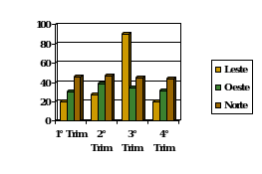
\includegraphics{imagens/img-grafico.png}}
    \caption[Exemplo de apresentação de uma figura no texto]{Exemplo de apresentação de uma figura no texto \cite{meregali2004}.}
    \label{fig:grafico}
\end{figure}

\subsection{Citações de fonte nas figuras}

Se  buscada em alguma obra publicada, deve aparecer sempre na descrição da figura, entre parênteses ``\cite{meregali2004}''.

Observando que na LISTA DE FIGURAS a fonte não deve aparecer.

\section{Descrição das Tabelas}

Veja exemplo de formatação da Tabela \ref{tab:exemplo-texto} a seguir: a legenda aparece acima da tabela, a descrição deve ser centralizada, no número de identificação \ref{tab:exemplo-texto}, o número 2 corresponde ao capítulo onde se localiza a tabela e o número 1 a ordem da tabela dentro do capítulo, seguido de dois ponto, espaço e  breve descrição, que deve ter a \emph{primeira} letra em maiúsculo.

Observe que as laterais das tabelas são abertas. Isso torna a imagem mais limpa e clara. As tabelas do texto não devem exceder a margem.

\begin{table}[h]
    \caption{Exemplo de apresentação de uma tabela no texto}
    \begin{center}
        \begin{tabular}{ c | c | c }
            \hline
            Manga & Abacaxi & Morango \\
            \hline
            12 & 100.000,00 & 10.000,00 \\
            \hline
            12 & 10.000,00 & 100.000,00 \\
            \hline
        \end{tabular}
    \end{center}
    \legend{Fonte: \citeauthor{meregali2004}, \citeyear{meregali2004}, p. 356.}
    \label{tab:exemplo-texto}
\end{table}

\subsection{Citações de fonte nas tabelas}

Se buscada em alguma obra publicada, a citação deve aparecer sempre na descrição da mesma, mas, diferentemente das figuras, a parte abaixo das Tabelas é reservada para a indicação de fontes dos dados, de modo similar a uma nota de rodapé. Contendo autor, ano e página. Veja exemplo acima.

Observando que na LISTA DE TABELAS a fonte não deve aparecer.

\section{Título 2}

xxxxxxxxxx\-xxxxxxxxxx\-xxxxxxxxxx\-xxxxxxxxxx\-xxxxxxxxxx\-xxxxxxxxxx\-xxxxxxxxxx\-xxxxxxxxxx\-xxxxxxxxxx\-xxxxxxxxxx\-xxxxxxxxxx\-xxxxxxxxxx\-xxxxxxxxxx\-xxxxxxxxxx\-xxxxxxxxxx\-xxxxxxxxxx\-xxxxxxxxxx\-xxxxxxxxxx\-xxxxxxxxxx\-xxxxxxxxxx\-xxxxxxxxxx\-xxxxxxxxxx\-xxxxxxxxxx\-xxxxxxxxxx\-xxxxxxxxxx\-xxxxxxxxxx\-xxxxxxxxxx\-xxxxxxxxxx\-xxxxxxxxxx\-xxxxxxxxxx\-xxxxxxxxxx\-xxxxxxxxxx\-xxxxxxxxxx\-xxxxxxxxxx\-xxxxxxxx

\begin{figure}[h]
    \centerline{
\includegraphics{imagens/img-carro.png}}
    \caption{Outro exemplo de figura}
    \label{fig:carro}
\end{figure}

\subsection{Título 3}

xxxxxxxxxx\-xxxxxxxxxx\-xxxxxxxxxx\-xxxxxxxxxx\-xxxxxxxxxx\-xxxxxxxxxx\-xxxxxxxxxx\-xxxxxxxxxx\-xxxxxxxxxx\-xxxxxxxxxx\-xxxxxxxxxx\-xxxxxxxxxx\-xxxxxxxxxx\-xxxxxxxxxx\-xxxxxxxxxx\-xxxxxxxxxx\-xxxxxxxxxx\-xxxxxxxxxx\-xxxxxxxxxx\-xxxxxxxxxx\-xxxxxxxx

\begin{quote}Citações com mais de 3 linhas devem possuir mais 4 cm de margem, fonte 10 pt, justificada xxxxxxxxxx\-xxxxxxxxxx\-xxxxxxxxxx\-xxxxxxxxxx\-xxxxxxxxx xxxxxxxxxx\-xxxxxxxxxx\-xxxxxxxxxx\-xxxxxxxxxx\-xxxxxxxxxx\-xxxxxxxxxx\-xxxxxxxxxx\-xxxxxxxxxx\-xxxxxxxxxx\-xxxxxxxxxx\-xxxxxxxxxx\-xxxxxxxxxx\-xxxx.\end{quote}

\subsubsection{Subseção}

O nível 4 não aparece no sumário. xxxxxxxxxx\-xxxxxxxxxx\-xxxxxxxxxx\-xxx xxxxxxxxxx\-xxxxxxxxxx\-xxxxxxxxxx\-xxxxxxxxxx\-xxxxxxxxxx\-xxxxxxxxxx\-xxxxxxxxxx\-xxxxxxxxxx\-xxxxxxxxxx\-xxxxxxxxxx\-xxxxxxxxxx\-xxxxxxxxxx\-xxxxxxxxxx\-xxxxxxxxxx\-xxxxxxxxxx\-xxxxxxxxxx\-xxxxxxxxxx\-xxxxxxxxxx\-xxxxxxxxxx\-xxxxxxxxxx\-xxxxxxxxxx\-xxxxxxxxxx\-xxxxxxxxxx\-xxxxxxxxxx\-xxxxxxxxxx\-xxxxxxxxxx\-xxxxxxxxxx\-xxxxxxxxxx\-xxxxxxxxxx\-xxxxxxx.

\subsubsection{Outra subseção}

xxxxxxxxxx\-xxxxxxxxxx\-xxxxxxxxxx\-xxxxxxxxxx\-xxxxxxxxxx\-xxxxxxxxxx\-xxxxxxxxxx\-xxxxxxxxxx\-xxxxxxxxxx\-xxxxxxxxxx\-xxxxxxxxxx\-xxxxxxxxxx\-xxxxxxxxxx\-xxxxxxxxxx\-xxxxxxxxxx\-xxxxxxxxxx\-xxxxxxxxxx\-xxxxxxxxxx\-xxxxxxxxxx\-xxxxxxxxxx\-xxxxxxxxxx\-xxxxxxxxxx\-xxxxxxxxxx\-xxxxxxx.

\subsection{Segundo}

xxxxxxxxxx\-xxxxxxxxxx\-xxxxxxxxxx\-xxxxxxxxxx\-xxxxxxxxxx\-xxxxxxxxxx\-xxxxxxxxxx\-xxxxxxxxxx\-xxxxxxxxxx\-xxxxxxxxxx\-xxxxxxxxxx\-xxxxxxxxxx\-xxxxxxxxxx\-xxxxxxxxxx\-xxxxxxxxxx\-xxxxxxxxxx\-xxxxxxx.

\begin{figure}[h]
    \centerline{
\includegraphics{imagens/img-paris.png}}
    \caption{Terceira figura: Local das férias depois do Trabalho de Conclusão}
    \label{fig:paris}
\end{figure}

\subsection{Terceiro}

xxxxxxxxxx\-xxxxxxxxxx\-xxxxxxxxxx\-xxxxxxxxxx\-xxxxxxxxxx\-xxxxxxxxxx\-xxxxxxxxxx\-xxxxxxxxxx\-xxxxxxxxxx\-xxxxxxxxxx\-xxxxxxxxxx\-xxxxxxxxxx\-xxxxxxxxxx\-xxxxxxxx
